\section{Практична частина}
\subsection{Емірний підсилювач}
\setlength{\parindent}{4em}



\begin{figure}[ht]
\centering
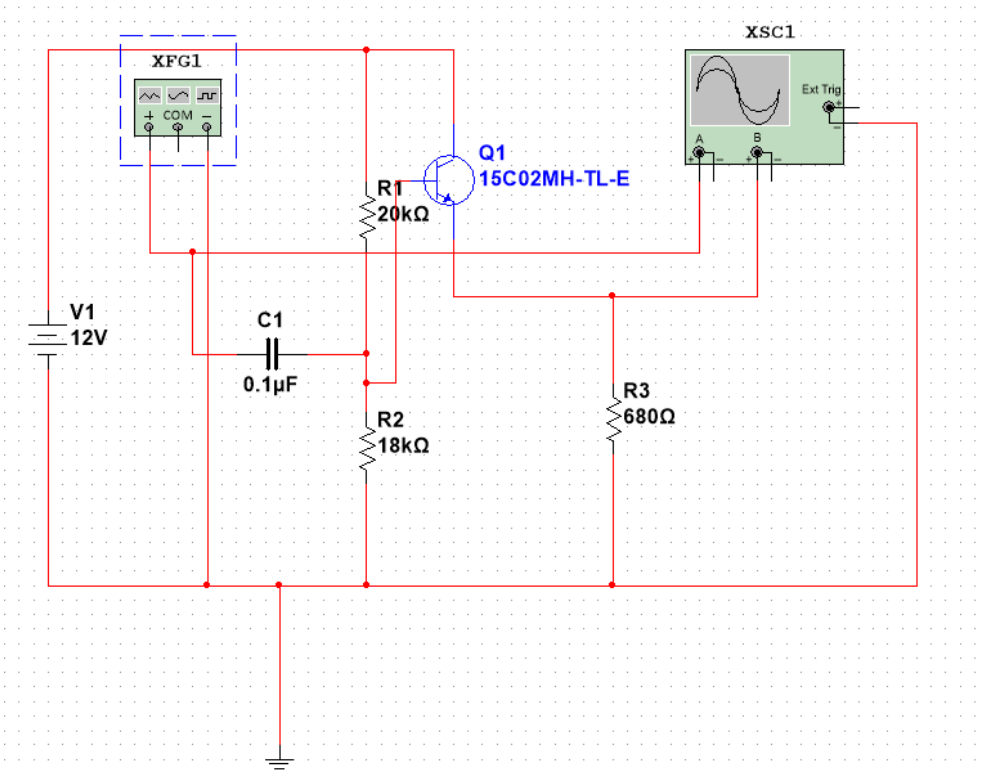
\includegraphics[width=0.7\linewidth]{Pic/first_1.png}
\end{figure}


\begin{figure}[ht]
\centering
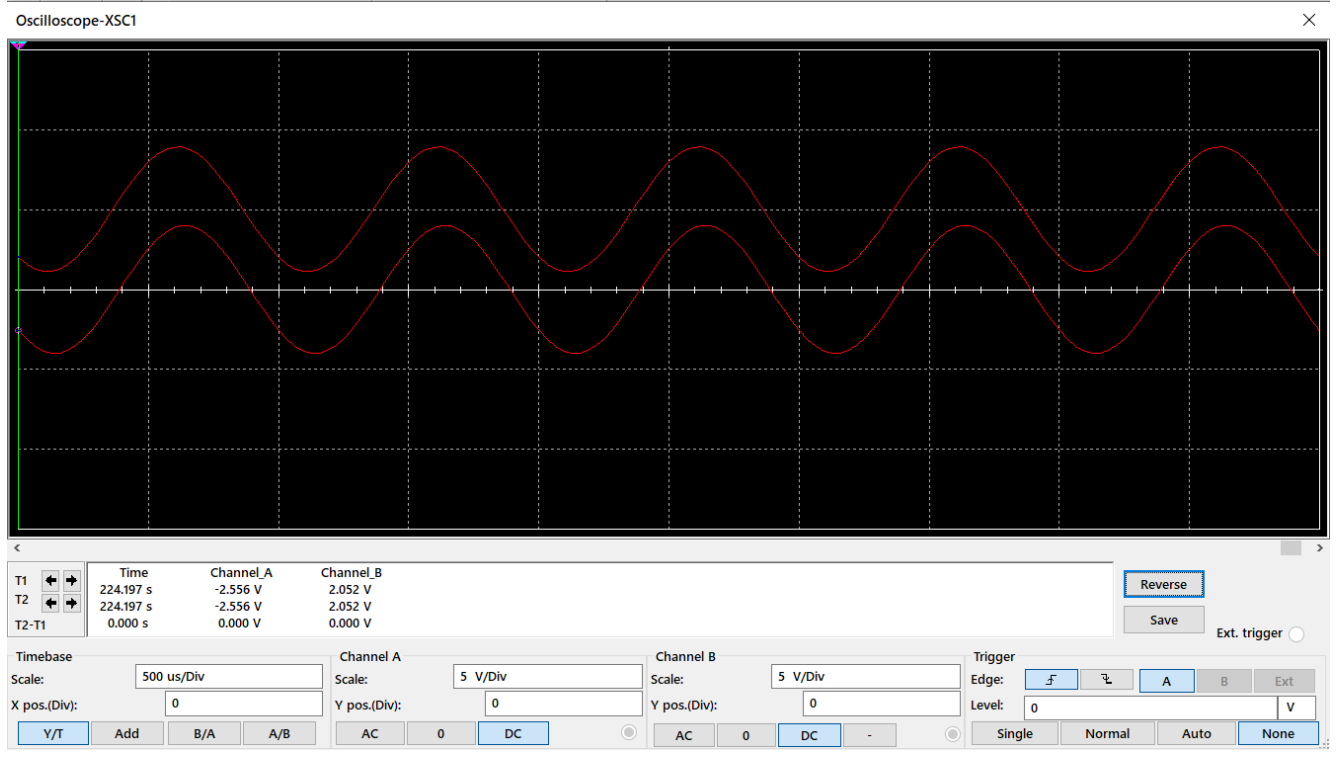
\includegraphics[width=0.9\linewidth]{Pic/first_2.png}
\end{figure}
\newpage

\subsection{Парфазний підсилювач}
\setlength{\parindent}{4em}



\begin{figure}[ht]
\centering
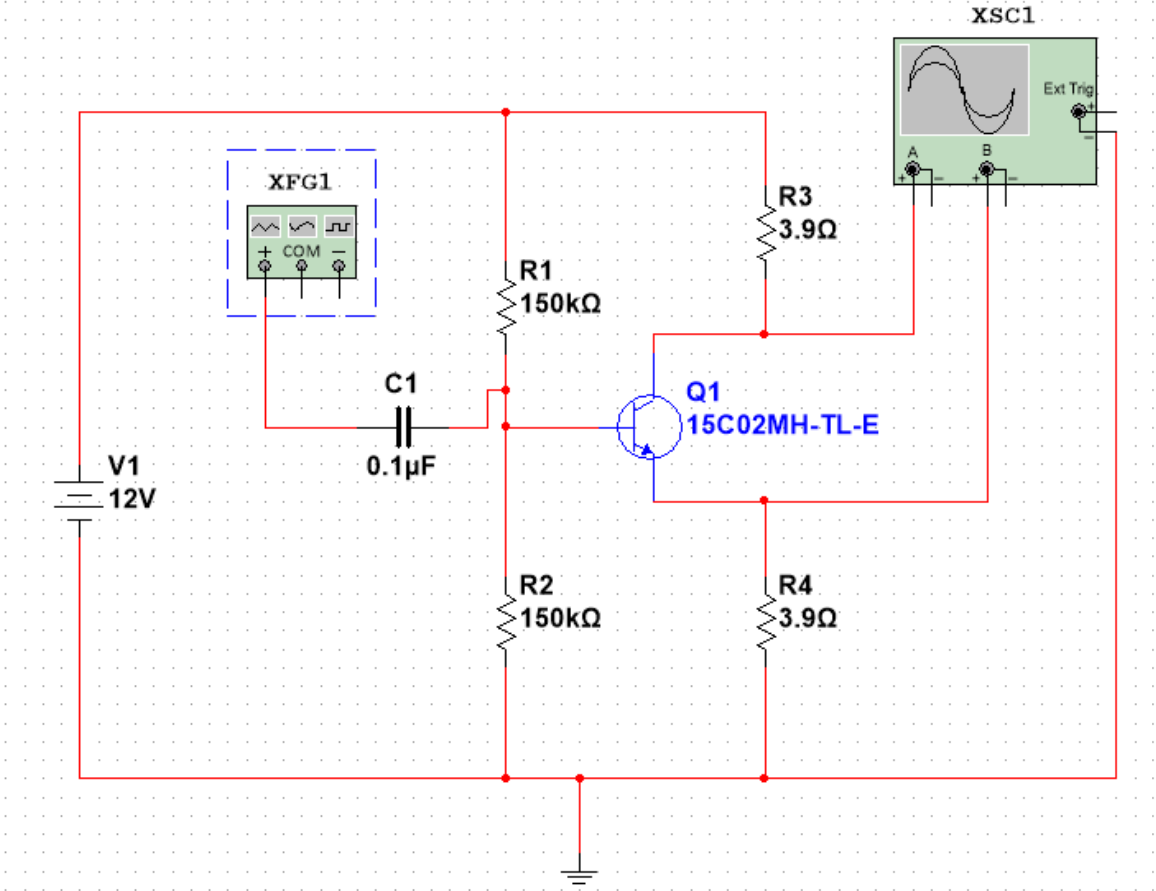
\includegraphics[width=0.7\linewidth]{Pic/second_1.png}
\end{figure}


\begin{figure}[ht]
\centering
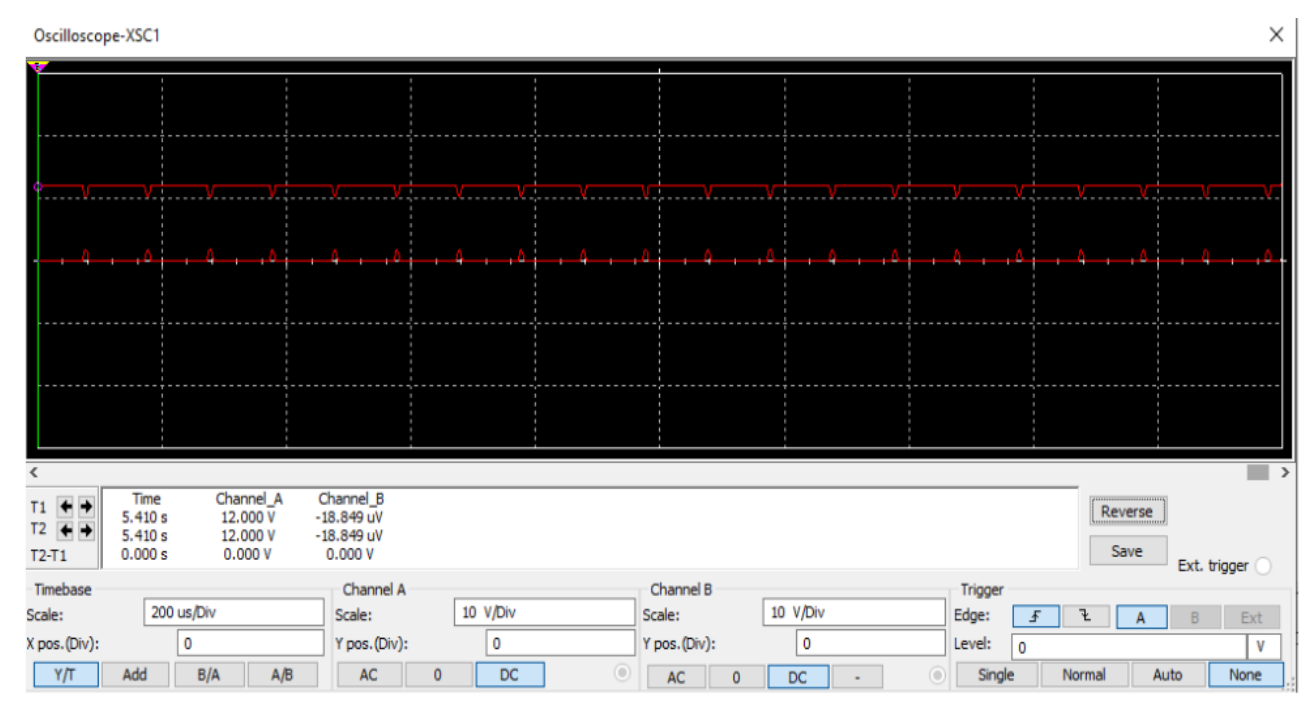
\includegraphics[width=0.9\linewidth]{Pic/second_2.png}
\end{figure}
\newpage

\subsection{ Підсилювач зі спільним емітером}
\setlength{\parindent}{4em}



\begin{figure}[ht]
\centering
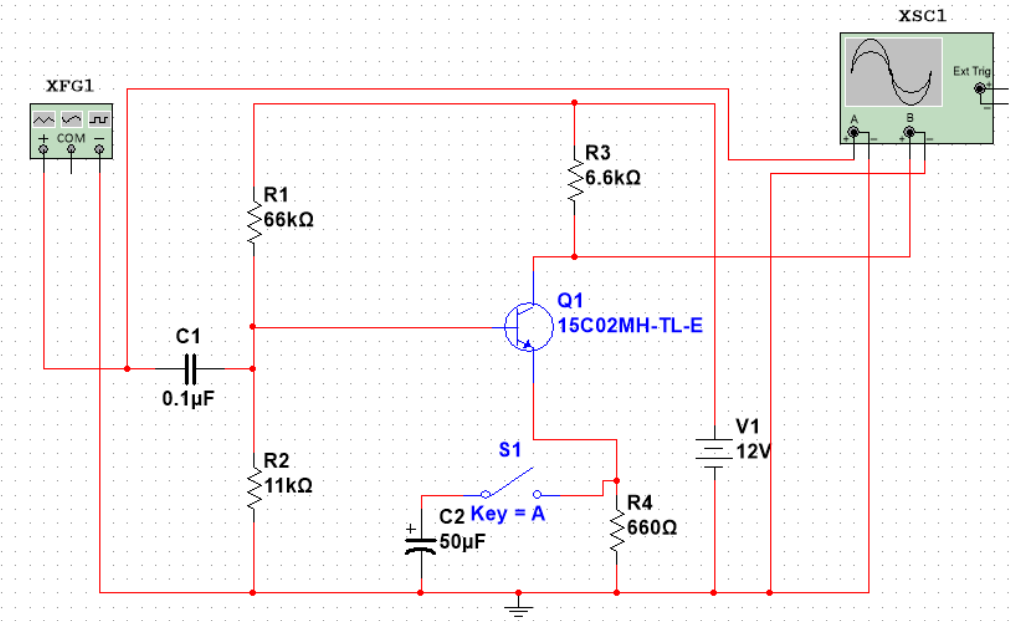
\includegraphics[width=0.5\linewidth]{Pic/third_1.png}
\end{figure}


\begin{figure}[ht]
\centering
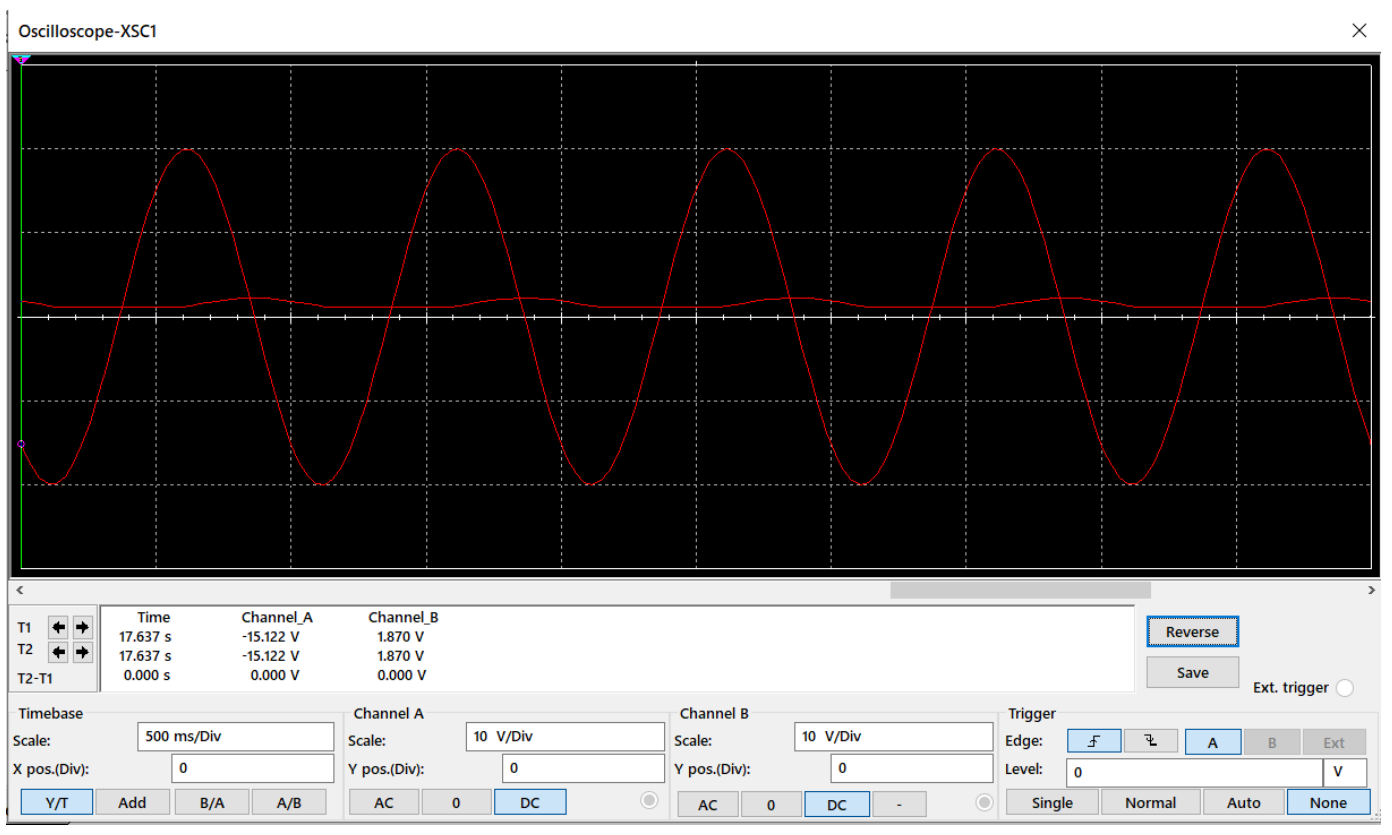
\includegraphics[width=0.6\linewidth]{Pic/third_2.png}
\end{figure}

\begin{figure}[ht]
\centering
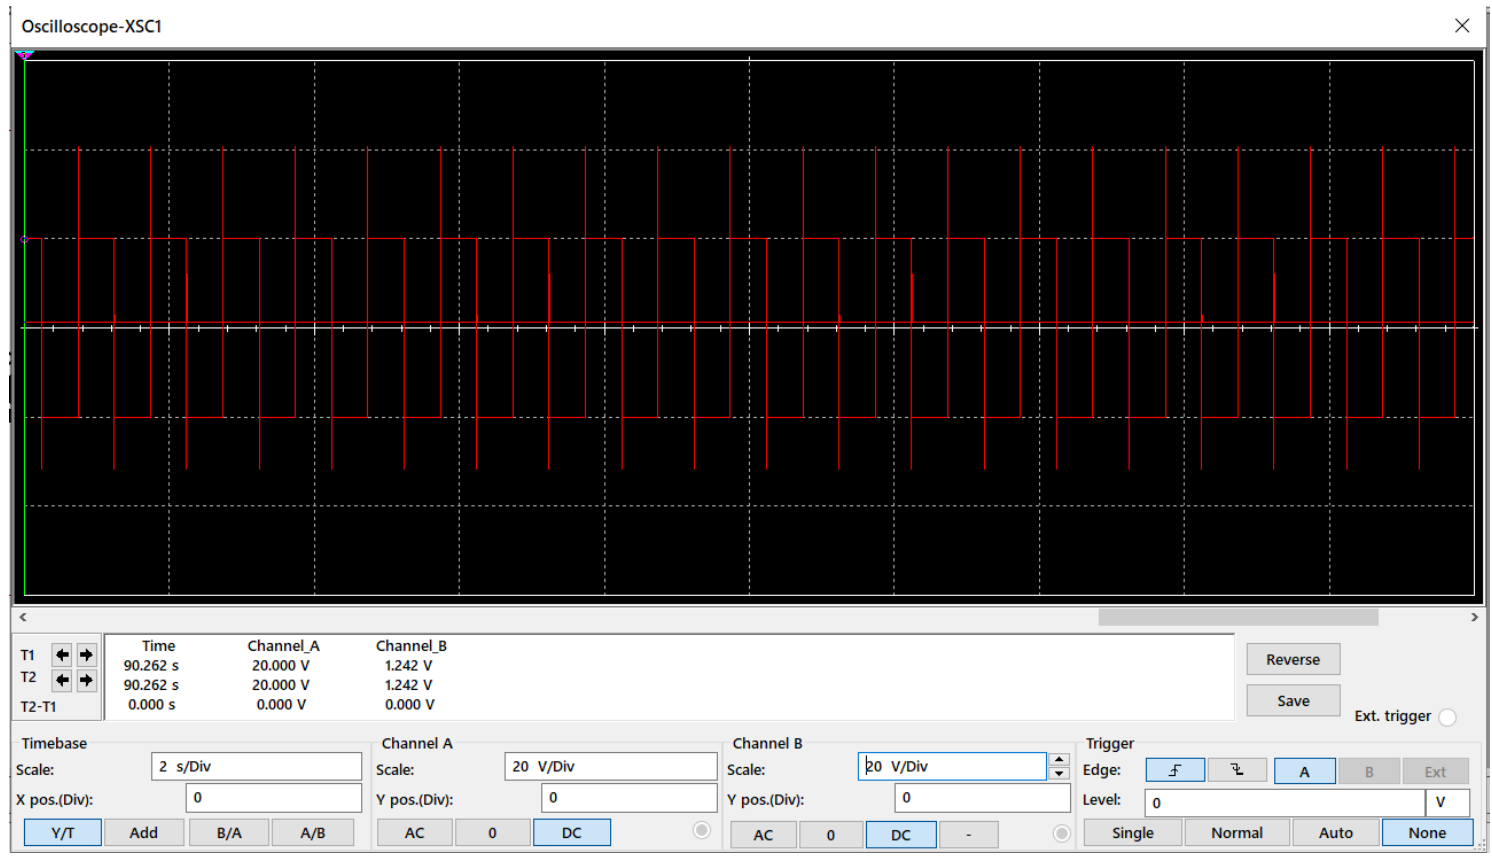
\includegraphics[width=0.6\linewidth]{Pic/third_3.png}
\end{figure}
\newpage

\subsection{Диференціальний підсилювач}
\setlength{\parindent}{4em}



\begin{figure}[ht]
\centering
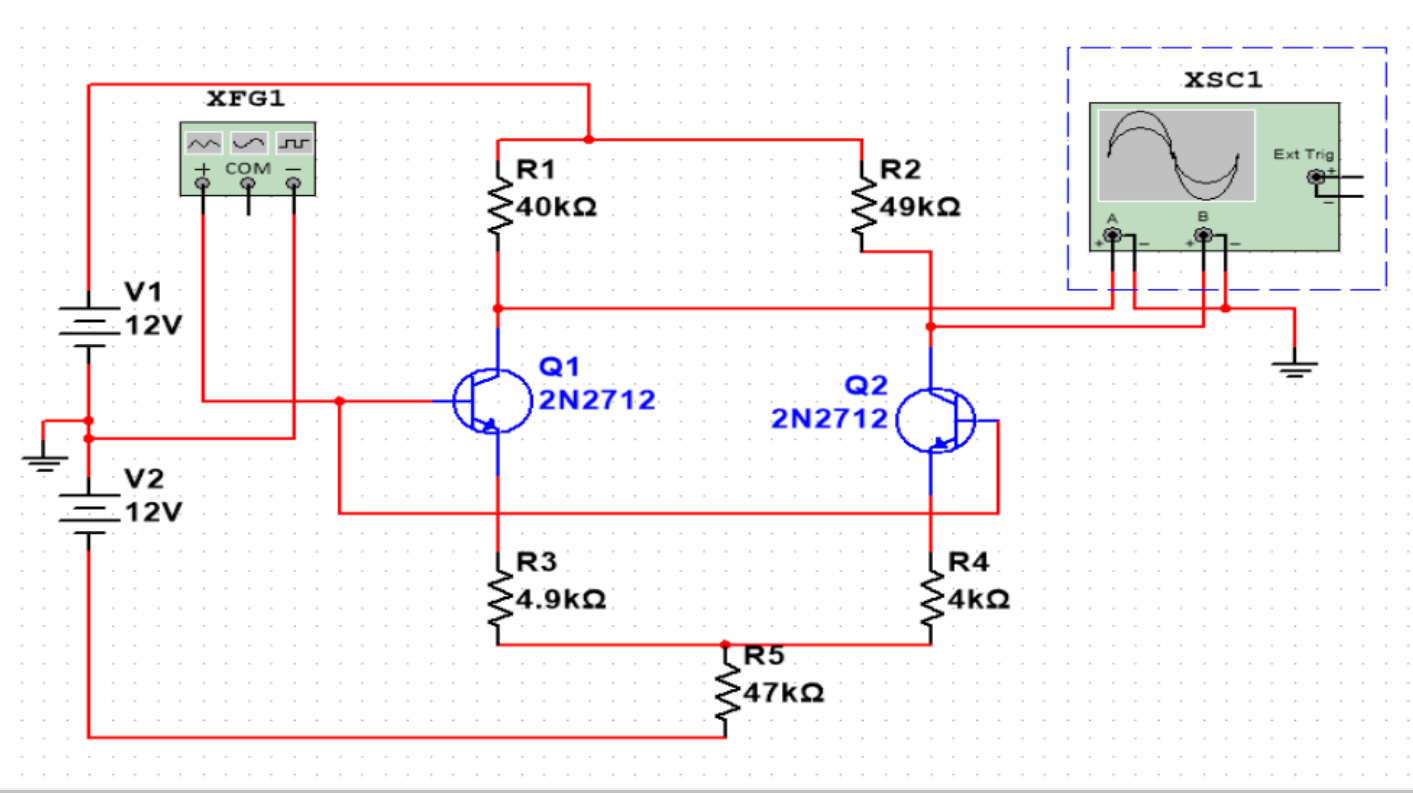
\includegraphics[width=0.6\linewidth]{Pic/4_1.png}
\end{figure}


\begin{figure}[ht]
\centering
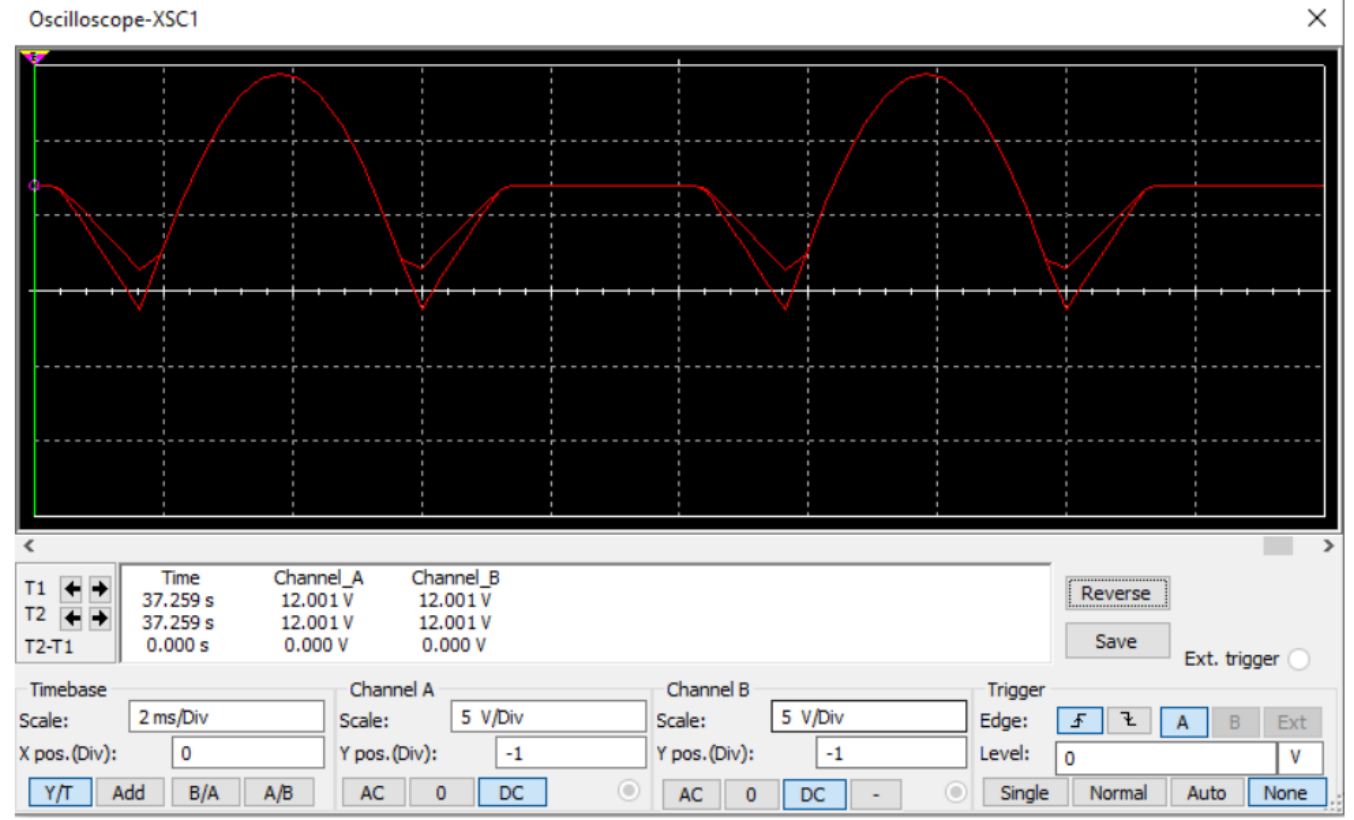
\includegraphics[width=0.7\linewidth]{Pic/4_2.png}
\end{figure}

\newpage
